\documentclass{beamer}

\usepackage{listings}

\usepackage[slovene]{babel}
\title{NRO DN1}
\author{Kristijan Danov}
\date{2024}


\begin{document}

\lstset{language=Matlab,%
    breaklines=true,
    morekeywords={matlab2tikz},
    keywordstyle=\color{blue},
    morekeywords=[2]{1}, keywordstyle=[2]{\color{black}},
    identifierstyle=\color{black},
    stringstyle=\color{mylilas},
    commentstyle=\color{mygreen},
    showstringspaces=false,
    emph=[1]{for,end,break},emphstyle=[1]\color{red}
}

\frame{\titlepage}

\begin{frame}
% \section{Kazalo}
\frametitle{Kazalo}
    \tableofcontents
\end{frame}

\begin{frame}
\section{$naloga1\_1.txt$}
\frametitle{$naloga1\_1.txt$}
    V $nalogi1\_1.txt$ imamo v prvi vrstici "$t[s]$", v drugi vrstici pa "stevilo preostalih  vrstic: 100; stevilo podatkov v vrstici: 1" \newline
    
    V drugih vrsticah imamo 100 časovnih točk, ki jih vnesemo v vektor $t$ s funkcijo importdata() v MATLAB-u.
\end{frame}

\begin{frame}
\section{Graf $P(t)$}
\frametitle{Graf $P(t)$}
    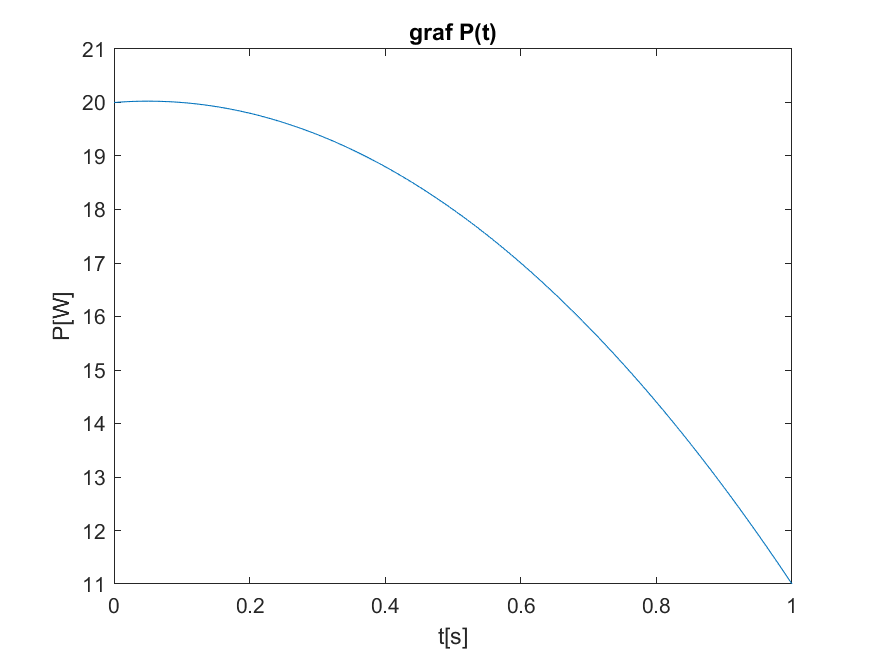
\includegraphics[width=0.9\textwidth]{graf.png}
    \centering
\end{frame}

\begin{frame}[fragile]
\section{Trapezna metoda}
\frametitle{Trapezna metoda}
    Formula za trapezna metoda: 
    \[\int_a^b f(x)dx = \frac{\Delta x}{2} (f(x_0)+2f(x_1)+2f(x_2)+...+2f(x_{n-1})+f(x_n))\]\
    \begin{lstlisting}[language=MatLab]
    sum = 0;
    for index = 1:size(P, 1)
    if index == 1 || index == size(P, 1)
        sum = sum + P(index);
    else
        sum = sum + 2*P(index);
    end
    end
    step = t(2) - t(1);
    integRes = (step/2)*sum
    
    \end{lstlisting}

    Rezultat smo dobili: $17.1665$
\end{frame}

\end{document}